\documentclass{beamer}
\usetheme{Warsaw}

\usepackage[utf8]{inputenc}
\usepackage{fancybox}
\usepackage{multimedia} 
\usepackage{subfig}
\usepackage{amsmath}
\usepackage{hyperref}
\usepackage[all]{xy}
\begin{document}


\title[Stochastik] % (optional, only for long titles)
{Stochastik für Informatiker
\\
\includegraphics[scale=0.5]{img/craps}
}
\subtitle{}
\author[Dr. Johannes Riesterer] % (optional, for multiple authors)
{Dr. rer. nat. Johannes Riesterer}

\date[KPT 2004] % (optional)
{}

\subject{Stochastik}

\frame{\titlepage}

\begin{frame}
    \frametitle{Übungsaufgaben}
\framesubtitle{}
\begin{block}{Aufgabe}
Einer Ihrer Bekannten behauptet, einen intelligenten Roboter gebaut zu haben. Um dies zu überprüfen, stellen Sie dem Roboter $n=20$ Fragen, die er mit Ja oder Nein beantworten soll. Entwerfen Sie einen  statistischen Test auf Basis des Binomial-Modells,  aus dem hervorgeht, ab wie vielen richtig beantworteten Ja-Nein-Fragen $c$ man mit einer Irrtumswahrscheinlichkeit von $0.05$ davon ausgehen kann, dass der Roboter tatsächlich intelligent ist und nicht nur zufällig die Antworten geraten hat. 
\end{block}
\begin{block}{Aufgabe}
Welchen Effekt hat eine Erhöhung der Anzahl der Versuche $n$ auf Ihren Test?
\end{block}
 \end{frame}


\begin{frame}
    \frametitle{Lösung}
\framesubtitle{}
Wir wählen das Binomialmodell $(\mathcal{X}= \{ 0, \cdots, n\},  P(\mathcal{X}), P_\rho = B_{n, \rho} : \rho \in \Theta =  [\frac{1}{2}, 1] )$, wobei $P_\rho (\{k \})=  B_{n, \rho}(\{k\}) = \begin{pmatrix} n \\ k \end{pmatrix} \rho^k (1-\rho)^{n-k} $ die \href{https://de.wikipedia.org/wiki/Binomialverteilung}{\underline{Binomialverteilung}} bezeichnet. Wir testen die Nullhypothese $H_0: \rho \in \Theta_0$ gegen die Alternative $H_1: \rho \in \Theta_1$ mit $\theta_0 = \frac{1}{2}$ und $\Theta_1 = (\frac{1}{2}, 1]$. Als Signifikanzniveau wählen wir $\alpha = 0.05$ und als Statistik wählen wir die Identität $T(x) = x$. Als Testfunktion wählen wir $\varphi = 1_{ \{ c, \cdots, n \}}$ und müssen $c \in \mathcal{X}$ so wählen, dass $\sup_{\rho \in \Theta_0} \mathbb{E}(\varphi )  < \alpha$ gilt.  Wir ermitteln also $c-1$ als das $0.05$-Fraktil der Binomialverteilung und damit $c = 15$, da $P_{\frac{1}{2}} (x \geq15) = 1 -P_{\frac{1}{2}} (x \leq 14) \approx 1 - 0,9793 = 0.027$.

 \end{frame}


\begin{frame}
    \frametitle{Lösung}
\framesubtitle{}
Bei Erhöhung der Versuche $n$ nimmt die Macht des Tests zu. Der Fehler zweiter Art wird also kleiner und der Test kann besser detektieren, dass der Roboter intelligent ist, wenn er es tatsächlich ist.
\begin{figure}[htp]
\centering
$n=20  -> c= 15$ (durchgezogen),$ n=40 -> c = 27$ gestrichelt.
      \centering
    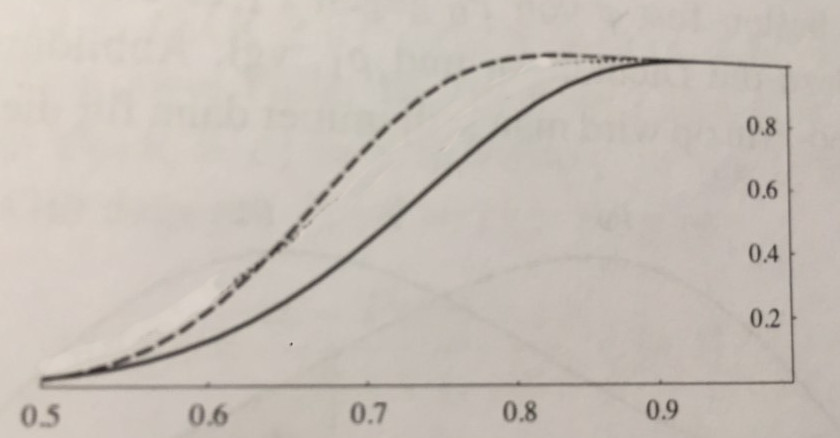
\includegraphics[width=0.7\textwidth]{img/bv}

      \caption{Quelle: Stochastik; Hans-OttoGeorgii}
\end{figure}

 \end{frame}



\end{document}
